\section{Procedimiento}

Se seleccionan cuatro varillas de distintas longitudes, se las mide y se arma
el péndulo de la fig. \ref{fig:procedimiento:esquema-pendulo}. Luego, utilizando
un cronómetro, se toma el tiempo que tarda el péndulo en realizar una
oscilación completa. Se repite esta medición 50 veces para cada varilla,
manteniendo siempre las mismas condiciones experimentales.

\begin{figure}[H]
    \centering
    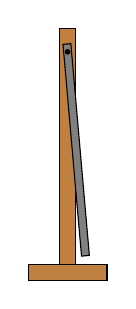
\begin{tikzpicture}
    \draw[fill=brown] (0,0) rectangle (1, 0.2);
    \draw[fill=brown] (0.4, 0.2) rectangle ++(0.2, 3);
    \draw[fill=gray, rotate around={5:(0.5, 2.9)}] (0.45, 3) rectangle 
    ++(0.1, -2.7);
    \filldraw[black] (0.5, 2.9) circle (0.8pt);
\end{tikzpicture}

    \caption{Esquema del péndulo físico}
    \label{fig:procedimiento:esquema-pendulo}
\end{figure}

Este arreglo permite que un extremo de la varilla quede anclado al dispositivo,
e impide su movimiento lateral. El eje en el que se inserta la
varilla contiene un rodamiento que permite que ésta rote con fricción
despreciable, lo que anula cualquier error que pudiera ser introducido por
fuerzas de rozamiento.
